\documentclass{beamer}
 \usepackage{subfigure}
\usepackage[utf8]{inputenc}
  \usepackage{tabu}
\usepackage{wrapfig,booktabs}
\usepackage{color}


 %\title[P-BPFS]{Physics-based preconditioners for large-
 %scale subsurface flow simulation.}
% 
% 
% \author[Diaz,Vuik,Jansen]
% {Gabriela Berenice Diaz Cortes \inst{1},
%   Prof. Kees Vuik \inst{1}, 
% Prof. J. D. Jansen \inst{2}}
% 
% \institute[TU Delft] % (optional)
% {
%   \inst{1}%
%   EWI\\
%   Delft University of Technology
%   \and
%   \inst{2}%
%   CiGT\\
%   Delft University of Technology
% }
 %\date{April 1st, 2016}
 %\logo{\includegraphics[height=0.5cm]{images/TU_Delft_logo.png}


%------------------------------------------------------------
%The next block of commands puts the table of contents at the 
%beginning of each section and highlights the current section:


\begin{document}
 
\frame{\titlepage}
%---------------------------------------------------------
%This block of code is for the table of contents after
%the title page
%\begin{frame}
%\frametitle{Table of Contents}
%\tableofcontents
%\end{frame}
%---------------------------------------------------------


\section{First section}
%---------------------------------------------------------
%Changing visivility of the text
\begin{frame}
\frametitle{Compressible problem}

To describe single-phase flow through a porous medium, the continuity equations are used:
\begin{equation}\label{eq:ce1}
\frac{\partial (\rho \phi)}{\partial t}- \nabla \cdot \left( \frac{\rho\mathbf{K}}{\mu}(\nabla \mathbf{p}-\rho g\nabla z)\right)=q.
\end{equation}
No rock compressibility is assumed $c_r=0$, fluid compressibility is assumed as constant:
\begin{equation}\label{eq:rhoeq}
 \rho(\mathbf{p})=\rho_0 e^{c_f(\mathbf{p}-\mathbf{p}_0)}.
\end{equation}
Well model\\
$$q=J(p_R-p_{bhp}),$$
where $J$ is the productivity or injectivity index.
\end{frame}
%----------------------------------------------------------------------
%---------------------------------------------------------
%Changing visivility of the text
\begin{frame}[shrink=20]
\frametitle{MRST solver}
Using implicit discretization:
\begin{equation}\label{eq:ce4}
 \frac{\mathbf{\phi}\mathbf{\rho}(\mathbf{p}^{n+1})
 -\mathbf{\phi}\mathbf{\rho}(\mathbf{p}^{n})}{\Delta t^n}
 -\nabla \cdot (\mathbf{\rho}(\mathbf{p}^{n+1}) 
 \frac{\mathbf{K}}{\mu}\nabla(\mathbf{p}^{n+1}))-{q}^{n}=0.
\end{equation}
$$q_{}^n=W_j(p_{r}^{n}-p_{bhp}^{n}).$$

The latter system can be written in short vector form as:
\begin{equation}\label{NR}
 \mathbf{F}(\mathbf{p}^{n+1};\mathbf{p}^n)=0,
\end{equation}
Newton-Rhapson linearization method, the $(n+1)$-th iteration approximation is obtained from:
$$\frac{\partial \mathbf{F}(\mathbf{p}^n)}{\partial \mathbf{p}^n}\delta\mathbf{p}^n=-\mathbf{F}(\mathbf{p}^n),
\qquad \delta \mathbf{p}^{n+1} =\mathbf{p}^{n+1}-\mathbf{p}^n,$$
where $\mathbf{J}(\mathbf{p}^n)=\frac{\partial \mathbf{F}(\mathbf{p}^n)}{\partial \mathbf{p}^n}$ is the 
Jacobian matrix, and $\mathbf{x}=\delta \mathbf{p}^{n+1}$ is the Newton update at iteration step $n+1$,
$\mathbf{b}=\mathbf{F}(\mathbf{p}^n)$ is the function evaluated at the time $n$.
The resulting system to solve is therefore:
$$\mathbf{J}\mathbf{x}=-\mathbf{b}.$$
\end{frame}
%----------------------------------------------------------------------
%---------------------------------------------------------
%Changing visivility of the text
\begin{frame}[shrink=35]
\frametitle{NR Algorithm}
\begin{tabular}[!ht]{|l|}
\hline
\hspace{0.5cm}\textbf{while} t $<$ totTime\\
 \hspace{1cm} $t = t + dt$\\ 
 \hspace{1cm}$step = step + 1$\\
  \hspace{1cm}\% Newton loop \\
 \hspace{1cm} $resNorm = 1e99$\\
 \hspace{1cm} $p0 = double(p_{ad})$ \hspace{2cm}\% Previous step pressure\\
 \hspace{1cm} $nit = 0$\\ \\
 \hspace{1cm} \textbf{while} (resNorm $>$ tol) \&\& (nit $<=$ maxits)\\
 \hspace{1.5cm}  \% Newton update\\
 \hspace{2cm}  $\mathbf{J}=eq.jac\{1\}$ \hspace{1.5cm}  \%Jacobian\\
\hspace{2cm}$res=eq.val$  \hspace{2cm} \%residual\\
\hspace{2cm} {\color{blue} resNorm = norm(res)}\\
\hspace{2cm}$upd=-(\mathbf{J}/res)$ {*}   
\hspace{1.5cm}\%Newton update, the solution of this system\\
\hspace{7cm}is obtained with ICCG or DICCG\\
  \hspace{1.5cm}  \% Update variables\\
\hspace{2cm}$p_{ad}.val+upd(pIx)$ \\
\hspace{2cm}$bhp_{ad}.val+upd(bhpIx)$  \\
\hspace{2cm}$qS_{ad}.val+upd(qsIx)$   \\
\hspace{2cm} resNorm = norm(res) \\
  \hspace{1.5cm}  $nit= nit + 1$\\
\hspace{1cm} \textbf{end}\\
\hspace{0.5cm}\textbf{end}\\
\hline
\end{tabular}
\end{frame}
%----------------------------------------------------------------------
% %---------------------------------------------------------
% %Changing visivility of the text
% \begin{frame}
% \frametitle{Solver}
% $$\mathbf{J}\mathbf{x}=-res.$$
% Stopping criterium of the iterative solver
% $$\frac{||\mathbf{M}^{-1}\mathbf{r}_{j+1}||_2}{||\mathbf{M}^{-1}\mathbf{b}||_2}.$$
% But 
% \begin{equation*}
%  \mathbf{F}(\mathbf{p}^{n+1};\mathbf{p}^n)=0,
% \end{equation*}
% therefore $\mathbf{F}(\mathbf{p}^n)$ is close to 0.
% %Then, a new stopping criteria must be used
% %$$\frac{||\mathbf{M}^{-1}\mathbf{r}_{j+1}||_2}{||\mathbf{M}^{-1}\mathbf{r}_0||_2}.$$
% %Drawback: depends on the initial guess ($\mathbf{x}_0$), 
% %however the initial guess used is $\mathbf{x}=\mathbf{0}.$
% \end{frame}
% %----------------------------------------------------------------------
%---------------------------------------------------------
%Changing visivility of the text
\begin{frame}[shrink=10]
\frametitle{System configuration}
\begin{itemize}
\begin{minipage}{.6\textwidth}
\item[]
\item[] Size: 35 x35 grid cells.
\item[] Initial pressure 200 bar.
 \item[]  W1 =  W2 = W3 = W4 = 100 bar.
 \item[] W5 = 600 bars.
 \item[] 10 Snapshots, same conditions \\(first set of experiments).\\
 \end{minipage}%
\begin{minipage}{.4\textwidth}
\item[] $Boundary$ $conditions:$\\
\item[] $\frac{\partial P(y=1)}{\partial n}=\frac{\partial P(y=ny)}{\partial n}=$
\item[] $\frac{\partial P(x=1)}{\partial n}=\frac{\partial P(x=nx)}{\partial n}=0$.

\end{minipage}
\begin{minipage}{.8\textwidth}
\item[] $Snapshots$ (second set of experiments).
 \item[] $\mathbf{z}_1$:  W2 = W3 = W4 =  100 bars, 
 W1 = 200 bars, W5 = 500 bars.
\item[] $\mathbf{z}_2$: W1 = W3 = W4 = 100 bars,
 W2 = 200 bars, W5 = 500 bars.
\item[] $\mathbf{z}_3$: W1 = W2 = W4 = 100 bars,
 W3 = 200 bars, W5 =  500 bars.
\item[] $\mathbf{z}_4$:  W1 = W2 = W3 = 100 bars,
 W4 = 200 bars, W5 =  500 bars.\\
\end{minipage}%
\end{itemize}

\end{frame}
%----------------------------------------------------------------------
%---------------------------------------------------------
%Changing visivility of the text
\begin{frame}[shrink=5]
\frametitle{Results}
\emph{\Large \textbf{Case 1}}
\begin{figure}[!h]
\centering 
\begin{minipage}{.45\textwidth}
 \centering
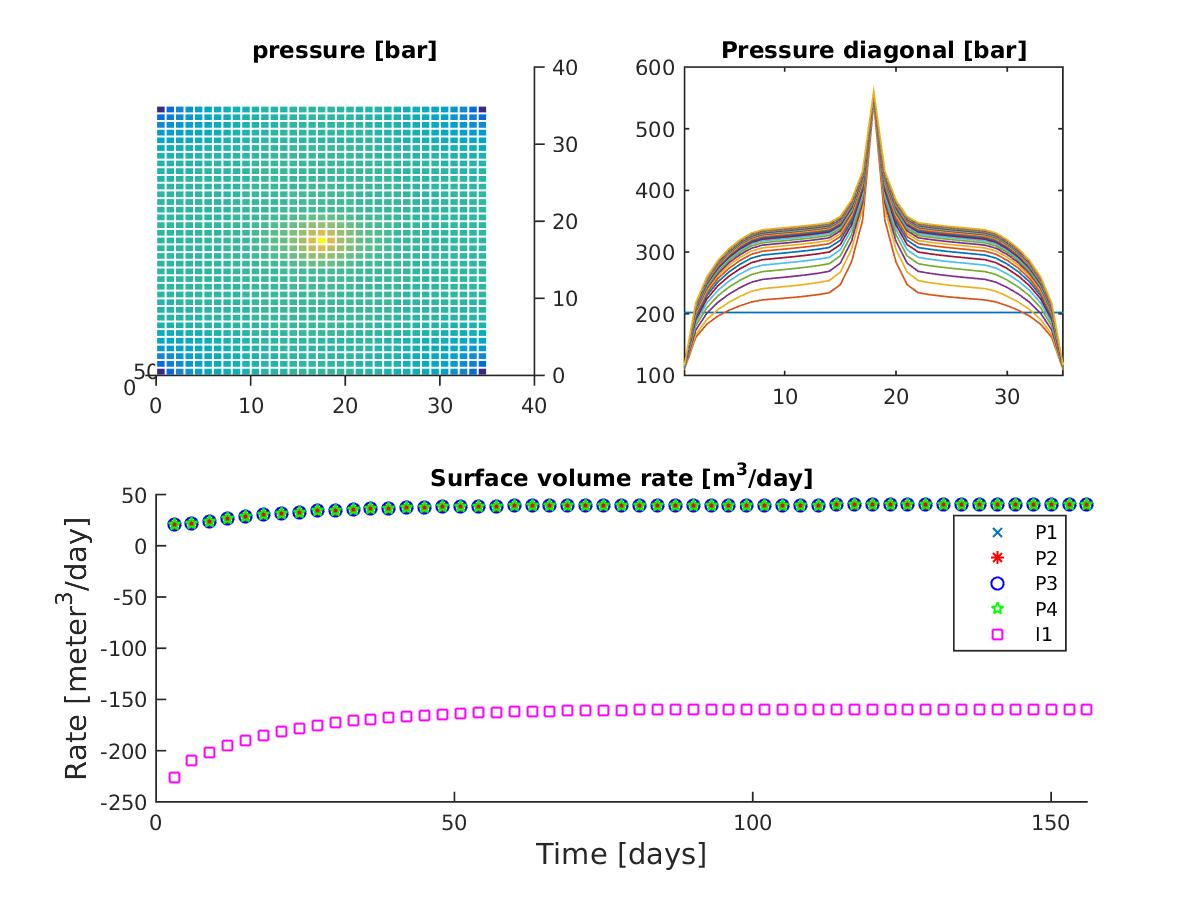
\includegraphics[width=6.5cm,height=6.5cm,keepaspectratio]{images/solutionIC.jpg}
\caption{Solution of the compressible problem solved with the ICCG method.}
\label{fig:compsol}
\end{minipage}%
\hspace{10mm}
\begin{minipage}{.45\textwidth}
 \centering
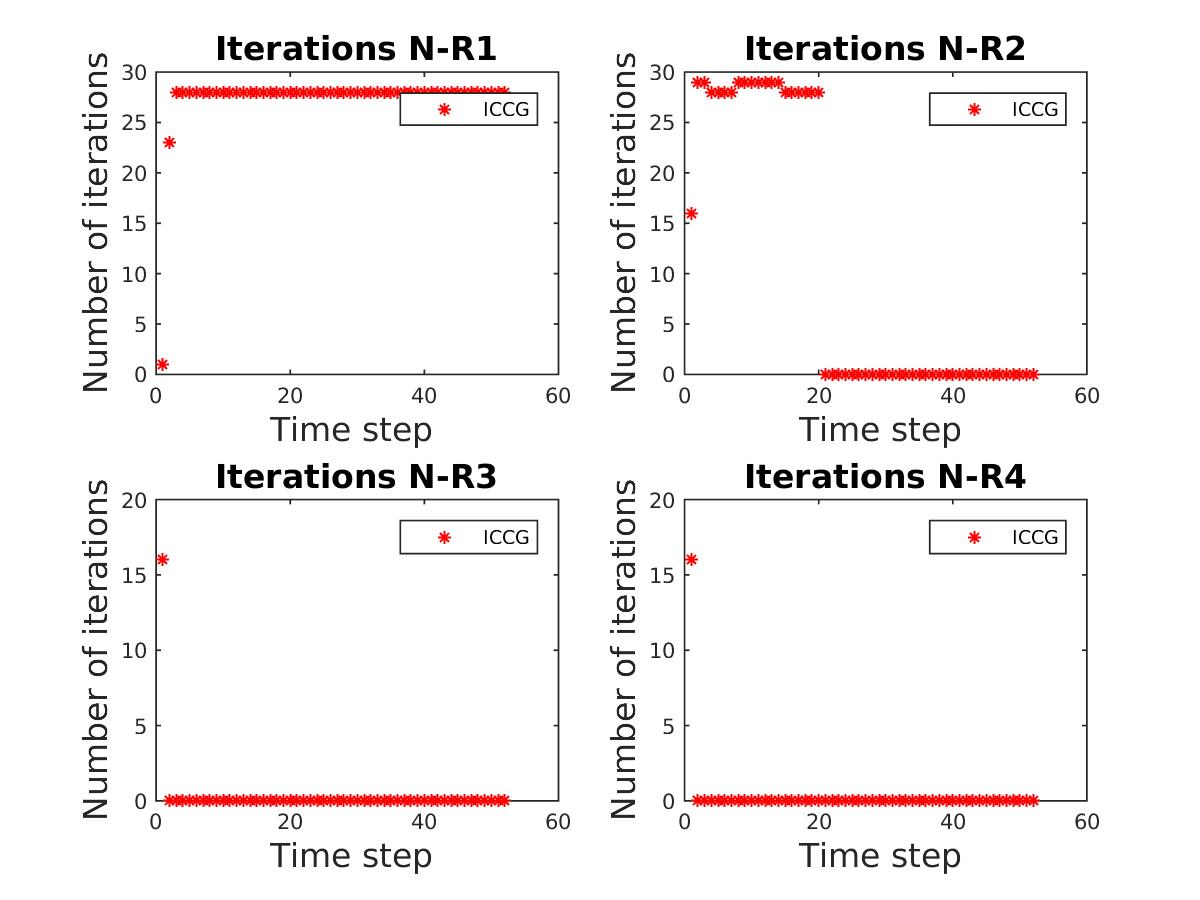
\includegraphics[width=6.5cm,height=6.5cm,keepaspectratio]
{images/iterations_4NR_IC.jpg}
\caption{Iterations, ICCG}
\label{fig:NR_IC}
\end{minipage}
\end{figure}
\begin{figure}[!h]
\centering
\begin{minipage}{.4\textwidth}
 \centering
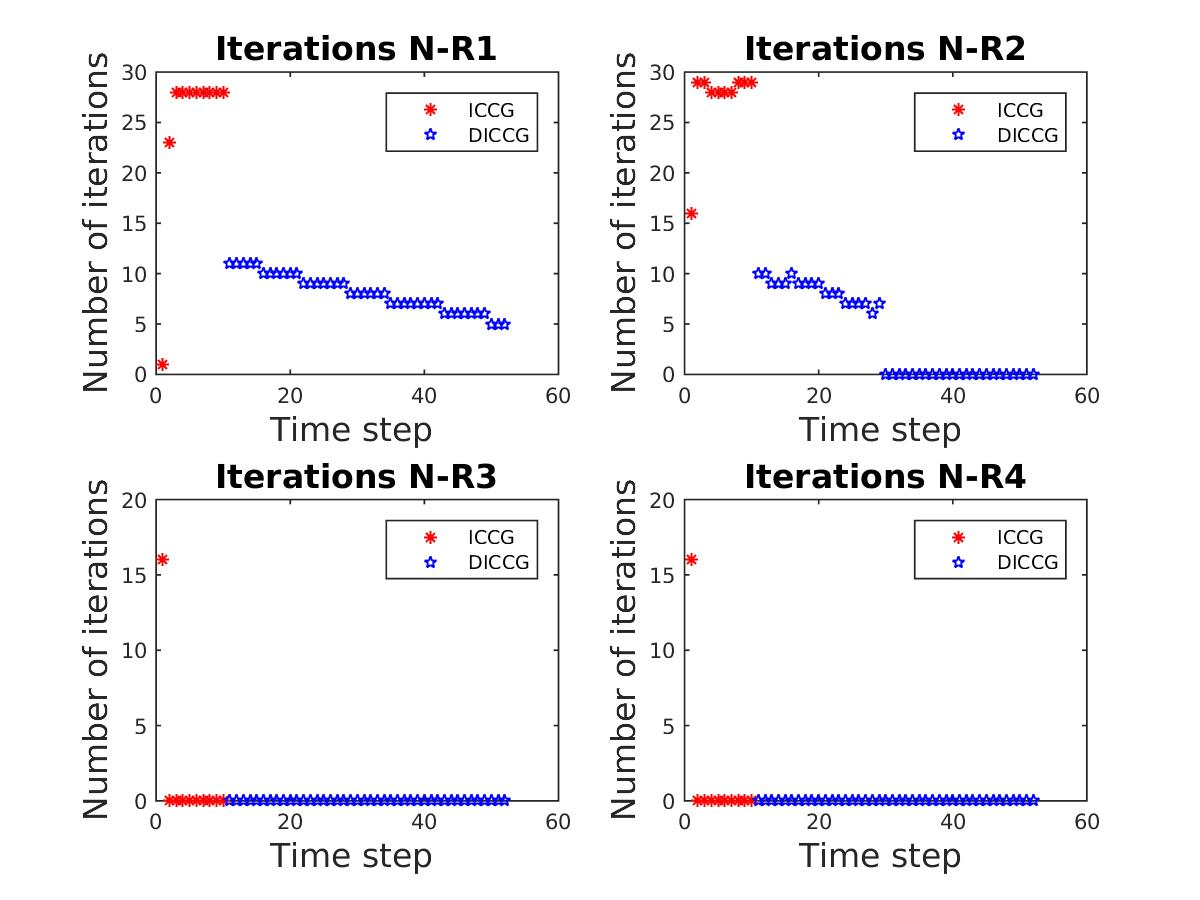
\includegraphics[width=6.5cm,height=6.5cm,keepaspectratio]
{images/iterations_4NR_D10.jpg}
\caption{Iterations DICCG$_{10}$}
\label{fig:NR_D10}
\end{minipage}%
\hspace{15mm}
\begin{minipage}{.4\textwidth}
 \centering
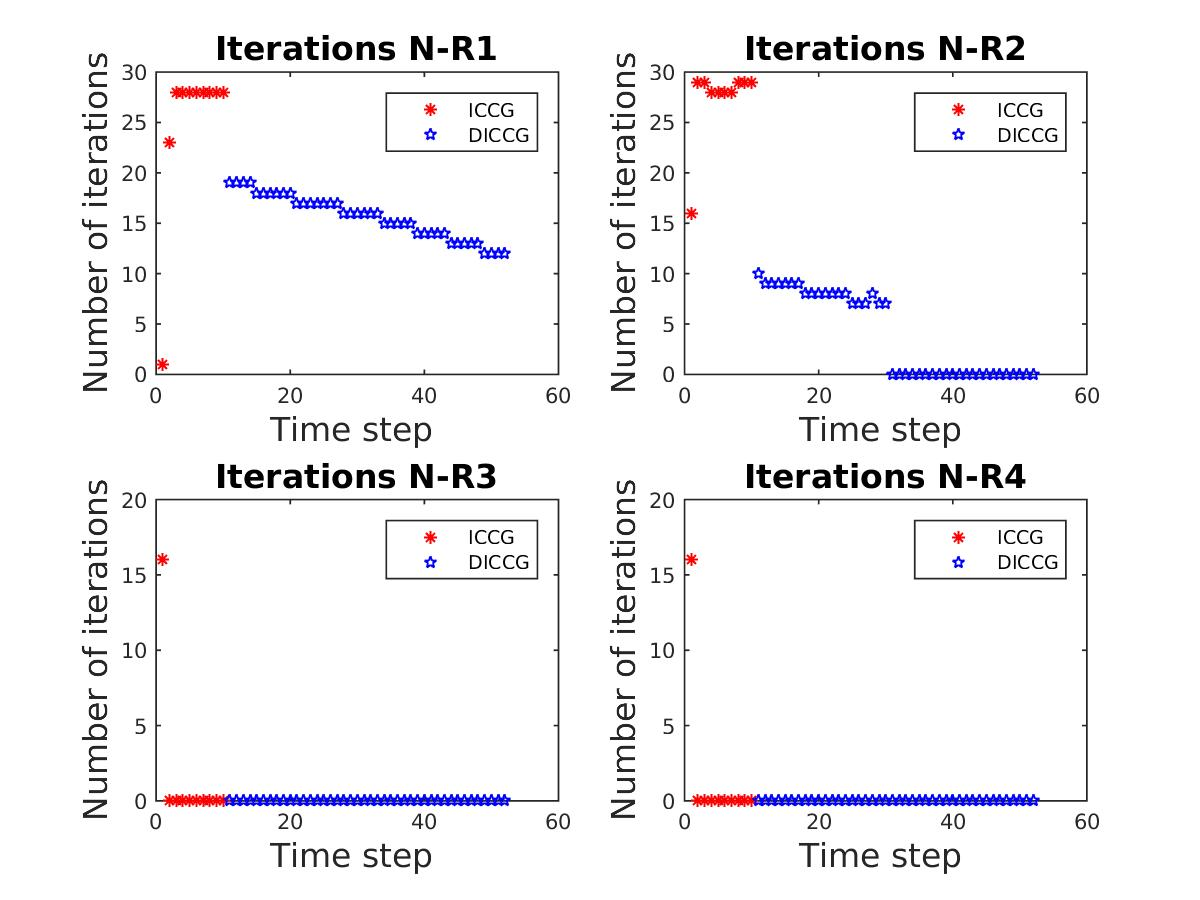
\includegraphics[width=6.5cm,height=6.5cm,keepaspectratio]
{images/iterations_4NR_POD5.jpg}
\caption{Iterations DICCG$_{5POD}$, 6-10}
\label{fig:NR_POD5}
\end{minipage}
\end{figure}
\end{frame}
%----------------------------------------------------------------------
%---------------------------------------------------------
%Changing visivility of the text
\begin{frame}[shrink=10]
\frametitle{Results}

\emph{\textbf{Case 1}}\\
\begin{figure}
\centering
\begin{minipage}{.45\textwidth}
 \centering
\includegraphics[width=6.5cm,height=6.5cm,keepaspectratio]{images/eigs1step.jpg}
\caption{eigs, step 1 A}
\label{fig:compsol}
\end{minipage}%
\hspace{10mm}
\begin{minipage}{.45\textwidth}
 \centering
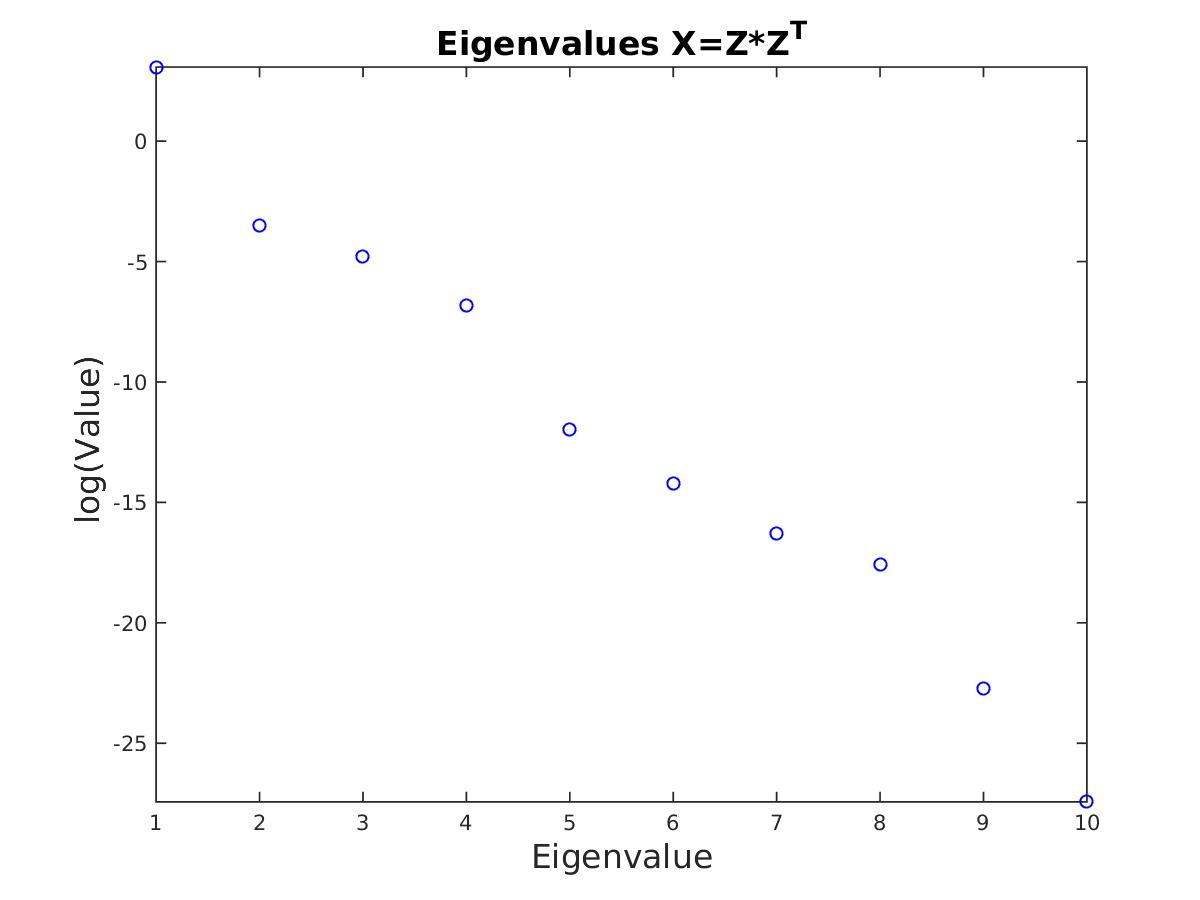
\includegraphics[width=6.5cm,height=6.5cm,keepaspectratio]
{images/eig_pod_10.jpg}
\caption{eigs POD, SVD}
\label{fig:NR_IC}
\end{minipage}
\end{figure}
\begin{figure}[!h]
\centering
\begin{minipage}{.4\textwidth}
 \centering
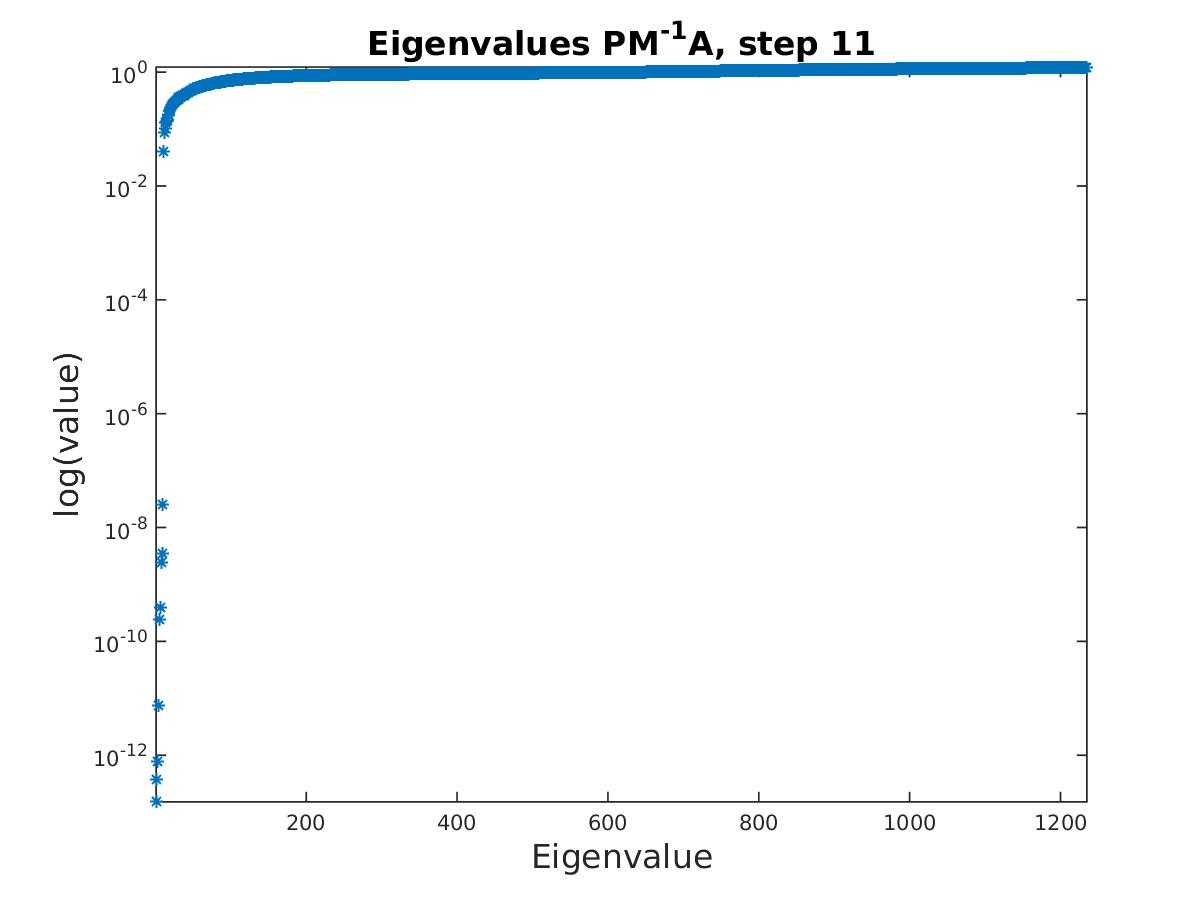
\includegraphics[width=6.5cm,height=6.5cm,keepaspectratio]
{images/eigsPA11step_D10.jpg}
\caption{eigs, step 11 PA}
\label{fig:NR_D10}
\end{minipage}%
\hspace{15mm}
\begin{minipage}{.4\textwidth}
 \centering
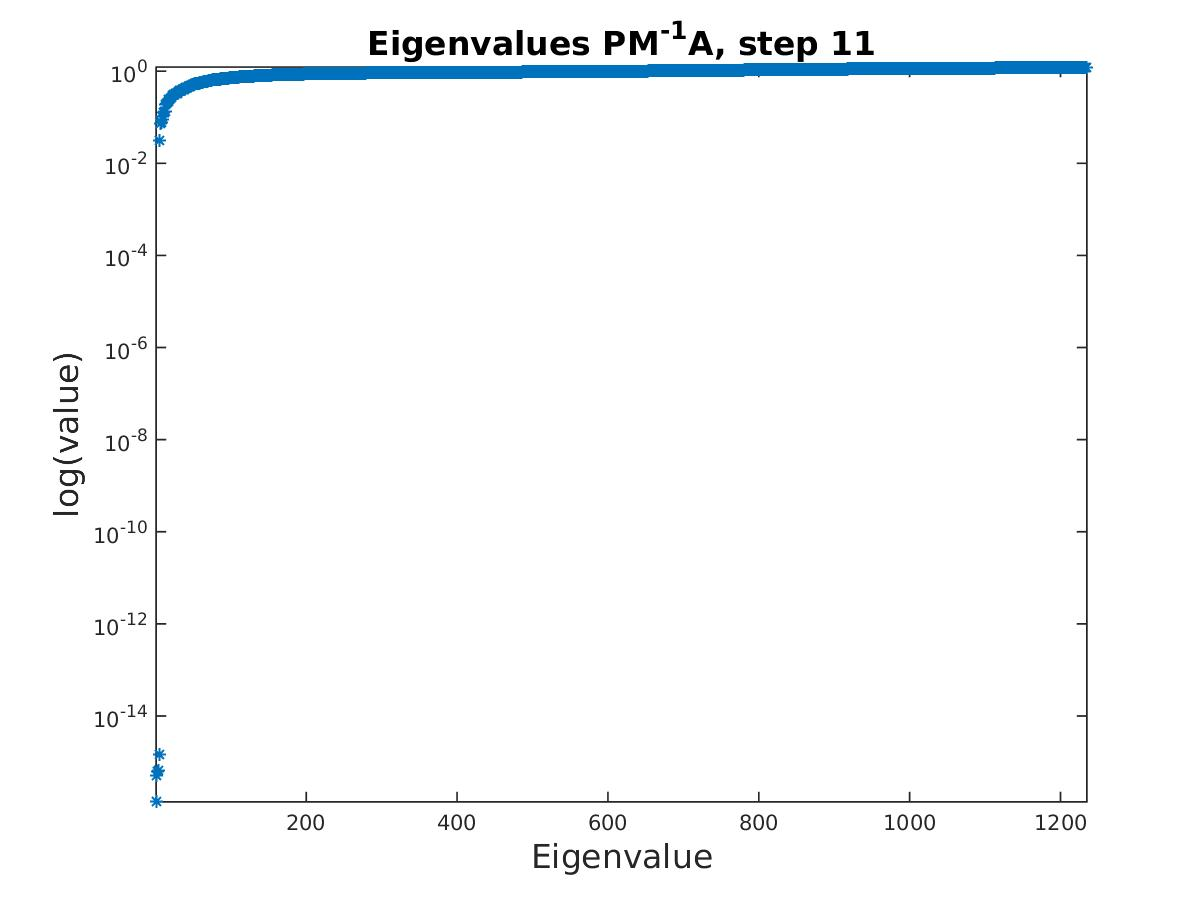
\includegraphics[width=6.5cm,height=6.5cm,keepaspectratio]
{images/eigsPA11step_POD5.jpg}
\caption{eigs, step 11 POD PA}
\label{fig:NR_POD5}
\end{minipage}
\end{figure}
\end{frame}
%---------------------------------------------------------

%---------------------------------------------------------
%Changing visivility of the text
\begin{frame}[shrink=5]
\frametitle{Results}
\emph{\Large \textbf{Case 1, $xi=x^{t-1}$}}\\
\begin{figure}[!h]
\centering 
\begin{minipage}{.45\textwidth}
 \centering
\includegraphics[width=6.5cm,height=6.5cm,keepaspectratio]
{/dev/media/Sphinx/Doctorado_Delft/Results/16_08/20/size_35perm_1_5wells_c_1e-3vxi/solution.jpg}
\caption{Solution of the compressible problem solved with the ICCG method.}
\label{fig:compsol}
\end{minipage}%
\hspace{10mm}
\begin{minipage}{.45\textwidth}
 \centering
\includegraphics[width=6.5cm,height=6.5cm,keepaspectratio]
{/dev/media/Sphinx/Doctorado_Delft/Results/16_08/20/size_35perm_1_5wells_c_1e-3vxi/iterations_4NR.jpg}
\caption{Iterations, ICCG}
\label{fig:NR_IC}
\end{minipage}
\end{figure}
\begin{figure}[!h]
\centering
\begin{minipage}{.4\textwidth}
 \centering
\includegraphics[width=6.5cm,height=6.5cm,keepaspectratio]
{/dev/media/Sphinx/Doctorado_Delft/Results/16_08/20/size_35perm_1_5wells_c_1e-3vxidv_10/iterations_4NR.jpg}
\caption{Iterations DICCG$_{10}$}
\label{fig:NR_D10}
\end{minipage}%
\hspace{15mm}
\begin{minipage}{.4\textwidth}
 \centering
\includegraphics[width=6.5cm,height=6.5cm,keepaspectratio]
{/dev/media/Sphinx/Doctorado_Delft/Results/16_08/20/size_35perm_1_5wells_c_1e-3vxidv_10/eigs/eigsPA11step.jpg}
\caption{Iterations DICCG$_{5POD}$, 1-5}
\label{fig:NR_POD5}
\end{minipage}
\end{figure}
\end{frame}
%----------------------------------------------------------------------



%---------------------------------------------------------
%Changing visivility of the text
\begin{frame}[shrink=5]
\frametitle{Results}
\emph{\Large \textbf{Case 1, problems}}\\
\begin{figure}[!h]
\centering 
\begin{minipage}{.45\textwidth}
 \centering
\includegraphics[width=6.5cm,height=6.5cm,keepaspectratio]
{/dev/media/Sphinx/Doctorado_Delft/Results/16_08/20/size_35perm_1_5wells_c_1e-3dv_5/iterations_4NR.jpg}
\caption{Iterations DICCG$_5$}
\label{fig:compsol}
\end{minipage}%
\hspace{10mm}
\begin{minipage}{.4\textwidth}
 \centering
\includegraphics[width=6.5cm,height=6.5cm,keepaspectratio]
{/dev/media/Sphinx/Doctorado_Delft/Results/16_08/20/size_35perm_1_5wells_c_1e-3dv_10pod12345/iterations_4NR.jpg}
\caption{Iterations DICCG$_{5POD}$, 1-5}
\label{fig:NR_POD5}
\end{minipage}
\end{figure}
\begin{figure}[!h]
\centering 
\begin{minipage}{.45\textwidth}
 \centering
\includegraphics[width=6.5cm,height=6.5cm,keepaspectratio]
{/dev/media/Sphinx/Doctorado_Delft/Results/16_08/20/size_35perm_1_5wells_c_1e-3dv_5/eigs/eigsPA6step.jpg}
\caption{Solution of the compressible problem solved with the ICCG method.}
\label{fig:compsol}
\end{minipage}%
\hspace{10mm}\begin{minipage}{.4\textwidth}
 \centering
\includegraphics[width=6.5cm,height=6.5cm,keepaspectratio]
{/dev/media/Sphinx/Doctorado_Delft/Results/16_08/20/size_35perm_1_5wells_c_1e-3dv_10pod12345/eigs/eigsPA11step.jpg}
\caption{Iterations DICCG$_{5POD}$, 1-5}
\label{fig:NR_POD5}
\end{minipage}
\end{figure}
\end{frame}
%----------------------------------------------------------------------





%---------------------------------------------------------
%Changing visivility of the text
\begin{frame}[shrink=5]
\frametitle{Results}
\emph{\Large \textbf{Case 2}}
\begin{figure}[!h]
\centering 
\begin{minipage}{.45\textwidth}
 \centering
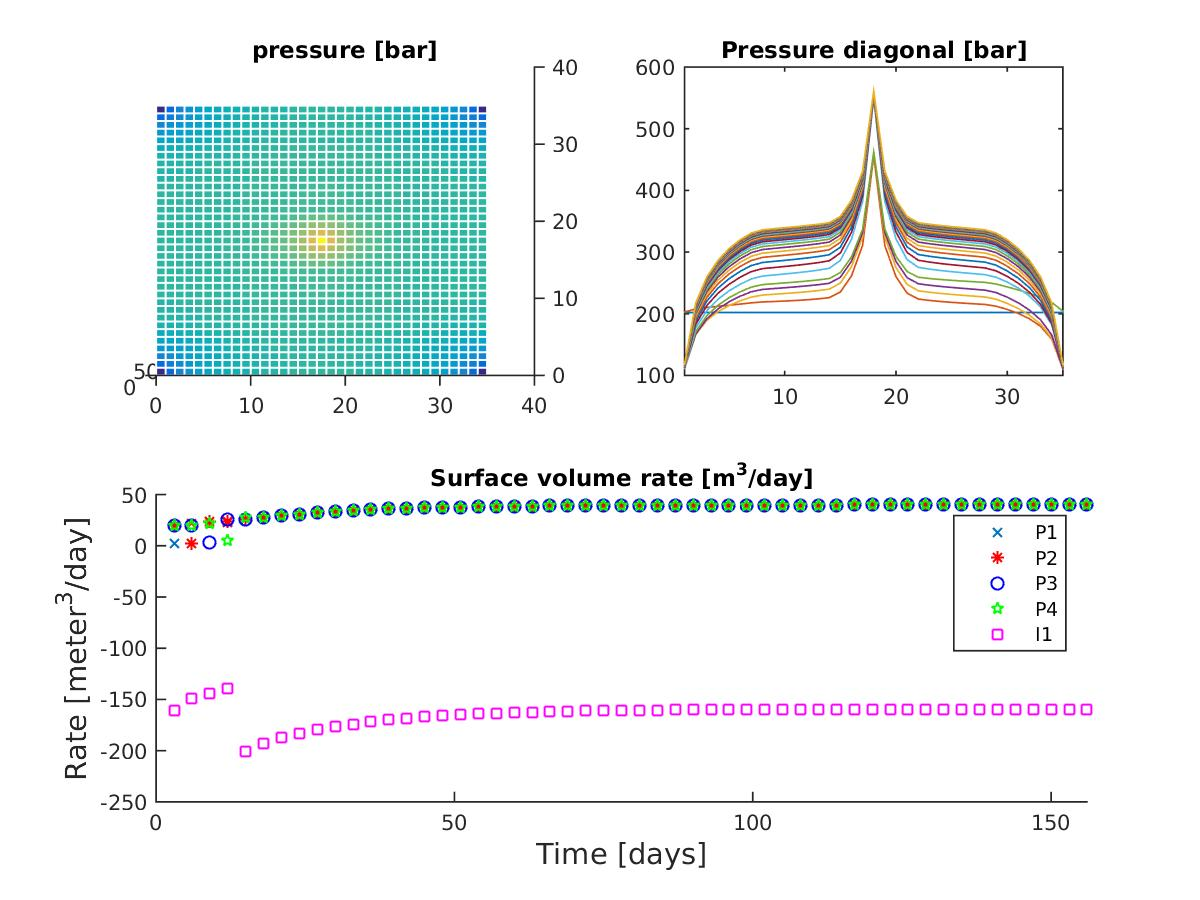
\includegraphics[width=6.5cm,height=6.5cm,keepaspectratio]{images/solutionvw_IC.jpg}
\caption{Solution of the compressible problem solved with the ICCG method.}
\label{fig:compsol}
\end{minipage}%
\hspace{10mm}
\begin{minipage}{.45\textwidth}
 \centering
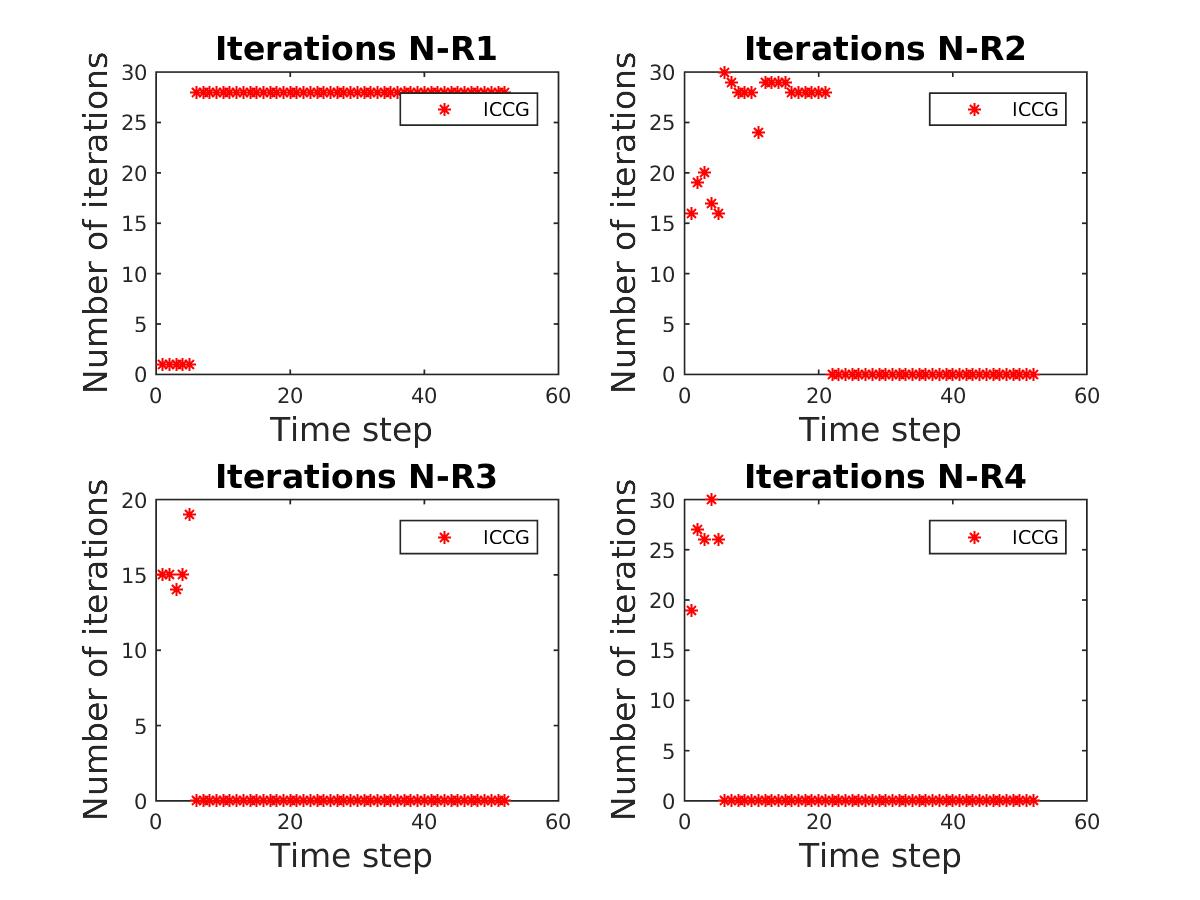
\includegraphics[width=6.5cm,height=6.5cm,keepaspectratio]
{images/iterations_4NRvw_IC.jpg}
\caption{Iterations, ICCG}
\label{fig:NR_IC}
\end{minipage}
\end{figure}
\begin{figure}[!h]
\centering
\begin{minipage}{.4\textwidth}
 \centering
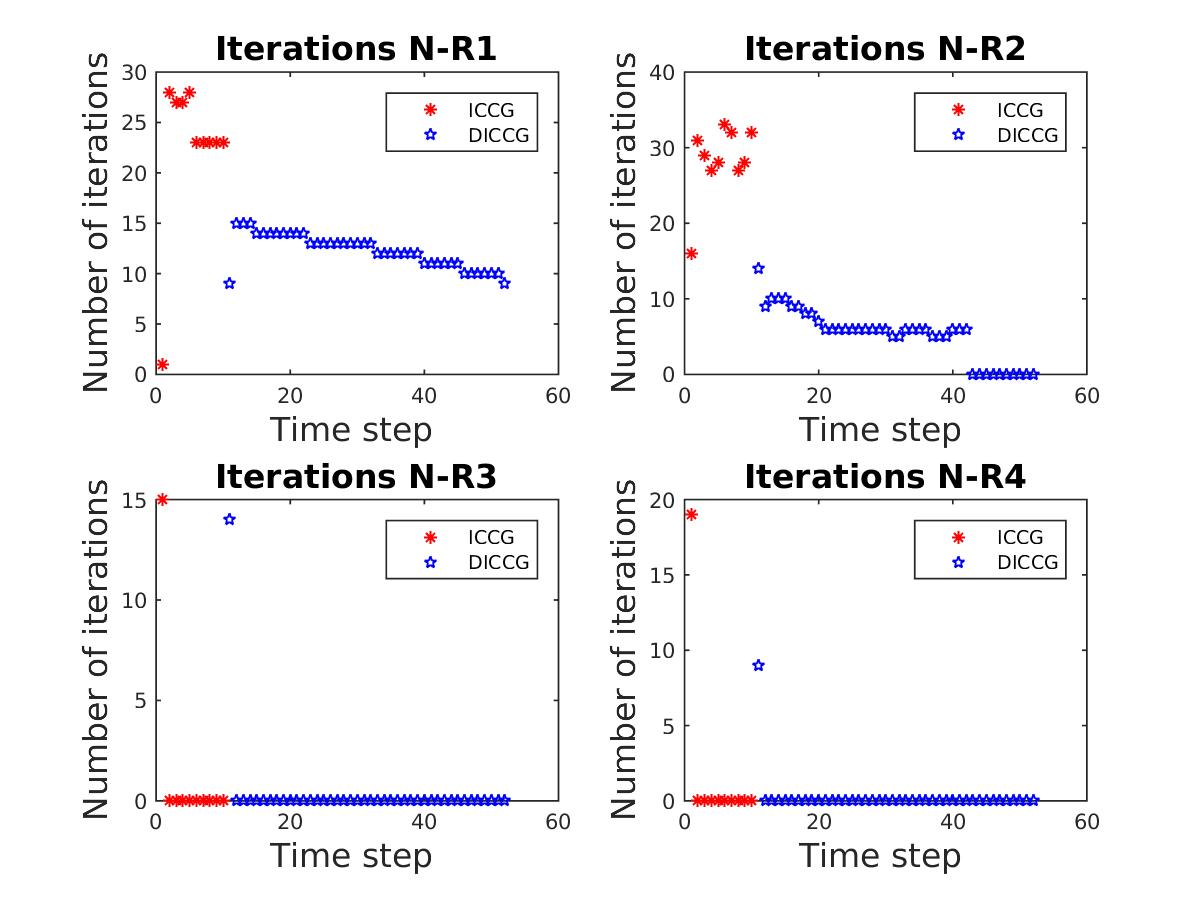
\includegraphics[width=6.5cm,height=6.5cm,keepaspectratio]
{images/iterations_4NRvw_D10.jpg}
\caption{Iterations DICCG$_{10}$}
\label{fig:NR_D10}
\end{minipage}%
\hspace{15mm}
\begin{minipage}{.4\textwidth}
 \centering
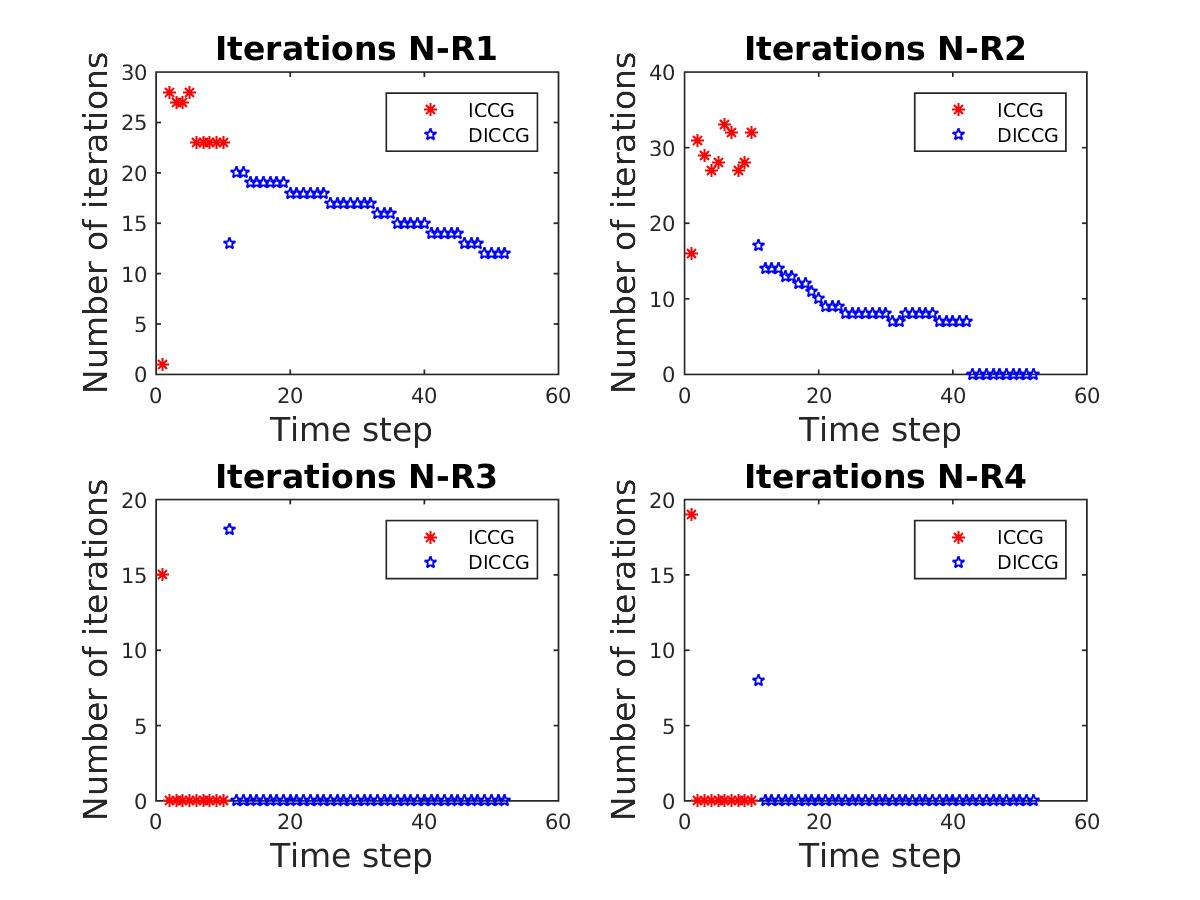
\includegraphics[width=6.5cm,height=6.5cm,keepaspectratio]
{images/iterations_4NRvw_POD5.jpg}
\caption{Iterations DICCG$_{5POD}$, 6-10}
\label{fig:NR_POD5}
\end{minipage}
\end{figure}
\end{frame}
%----------------------------------------------------------------------

%---------------------------------------------------------
%Changing visivility of the text
\begin{frame}[shrink=10]
\frametitle{Results}

\emph{\textbf{Case 2}}\\
\begin{figure}
\centering
\begin{minipage}{.45\textwidth}
 \centering
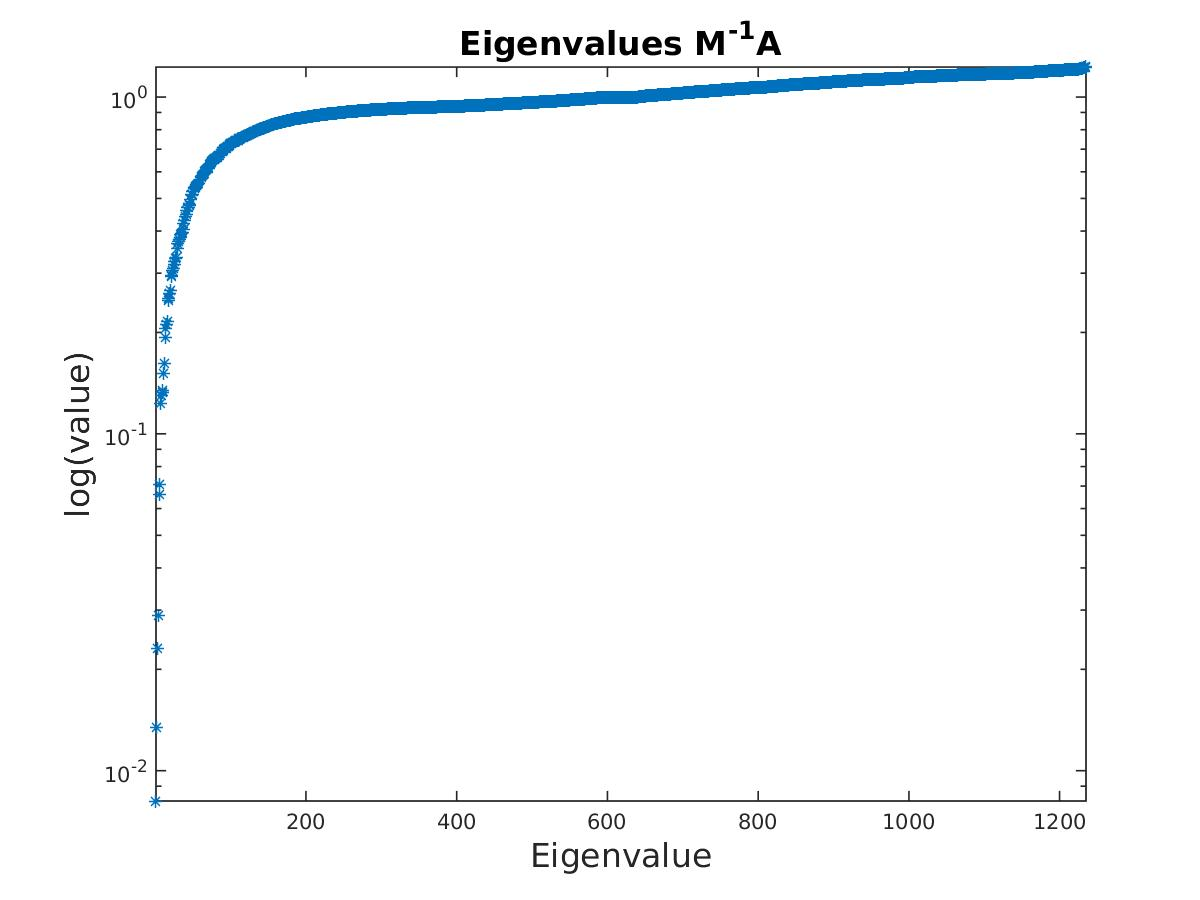
\includegraphics[width=6.5cm,height=6.5cm,keepaspectratio]{images/eigs1stepvw.jpg}
\caption{eigs, step 1 A}
\label{fig:compsol}
\end{minipage}%
\hspace{10mm}
\begin{minipage}{.45\textwidth}
 \centering
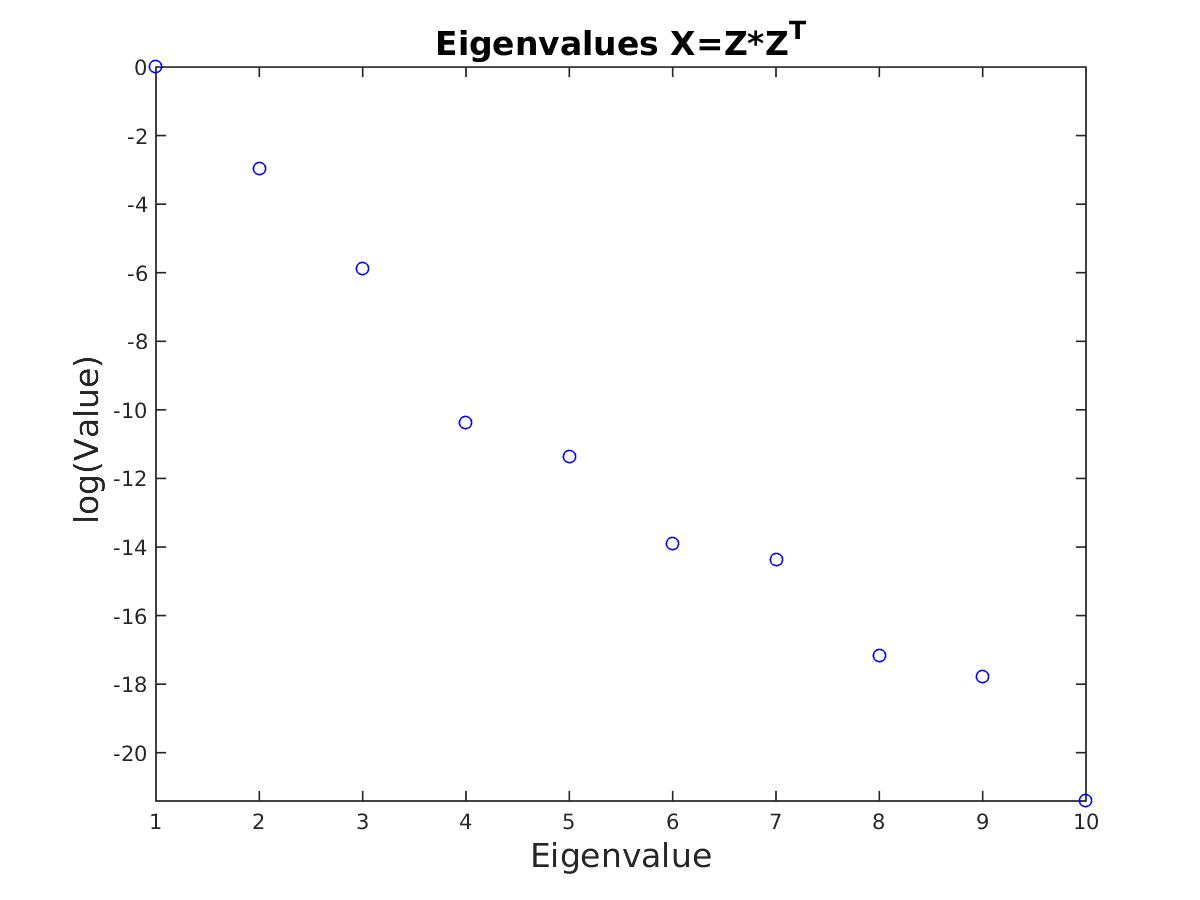
\includegraphics[width=6.5cm,height=6.5cm,keepaspectratio]
{images/eig_podvw_5.jpg}
\caption{eigs POD, SVD}
\label{fig:NR_IC}
\end{minipage}
\end{figure}
\begin{figure}[!h]
\centering
\begin{minipage}{.4\textwidth}
 \centering
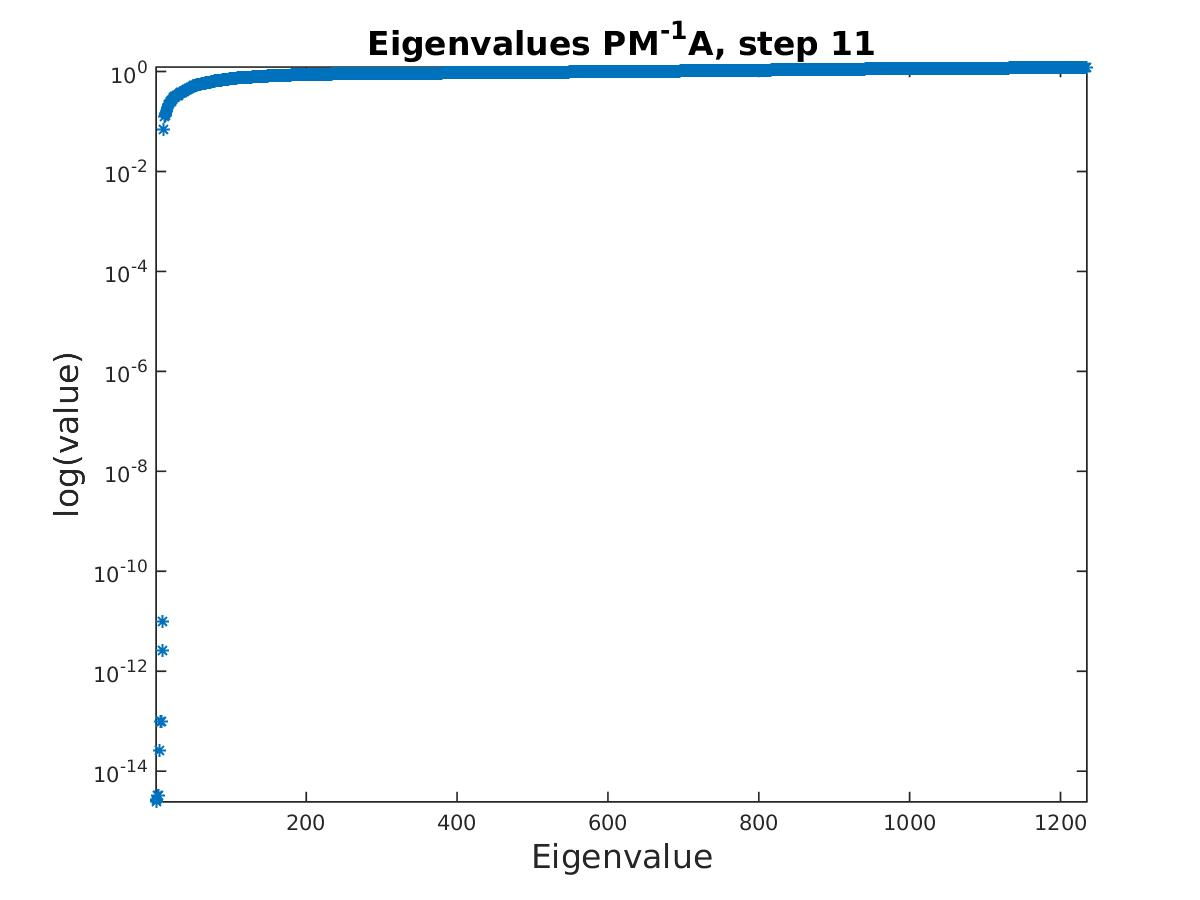
\includegraphics[width=6.5cm,height=6.5cm,keepaspectratio]
{images/eigsPA11stepvw_D10.jpg}
\caption{eigs, step 11 PA}
\label{fig:NR_D10}
\end{minipage}%
\hspace{15mm}
\begin{minipage}{.4\textwidth}
 \centering
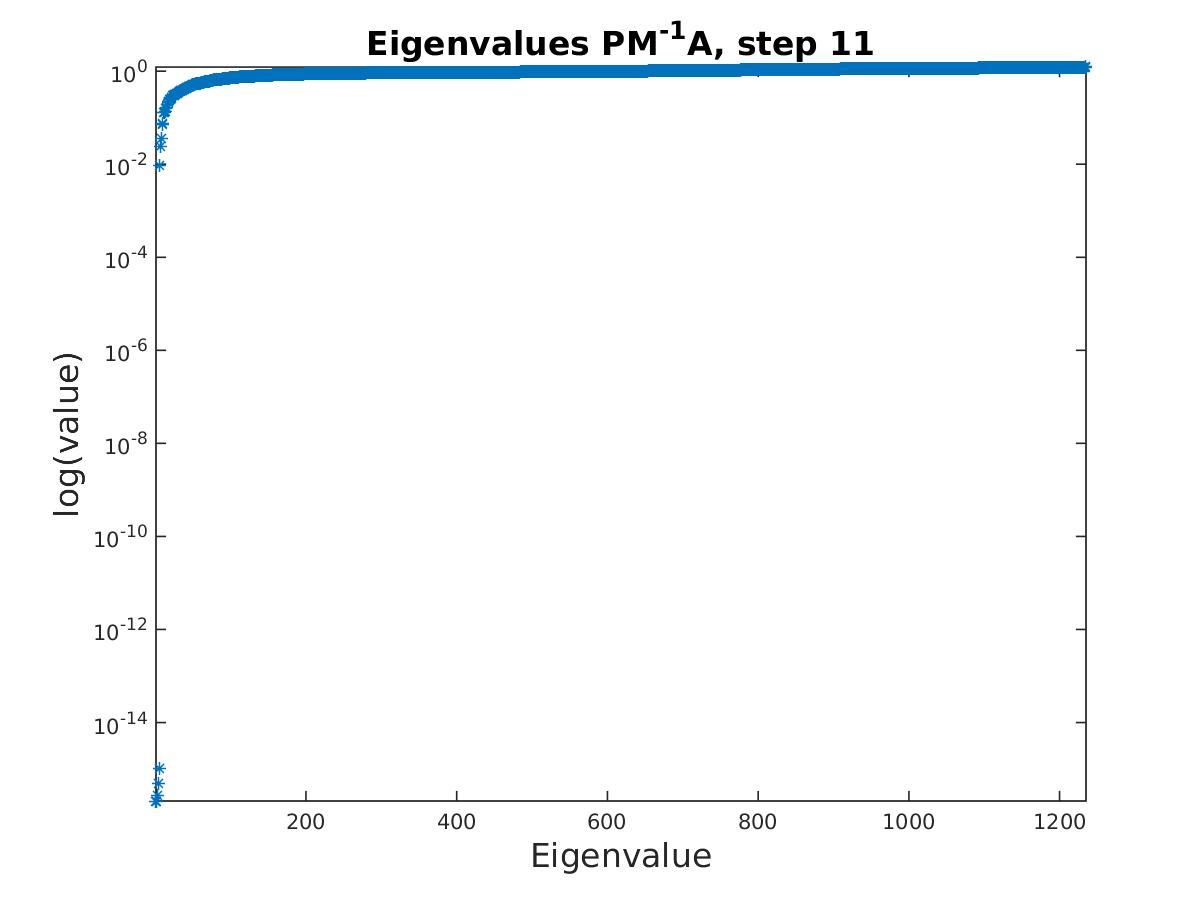
\includegraphics[width=6.5cm,height=6.5cm,keepaspectratio]
{images/eigsPA11stepvw_POD5.jpg}
\caption{eigs, step 11 POD PA}
\label{fig:NR_POD5}
\end{minipage}
\end{figure}
\end{frame}
%----------------------------------------------------------------------
%---------------------------------------------------------
%Changing visivility of the text
\begin{frame}[shrink=5]
\frametitle{Results}
\emph{\Large \textbf{SPE 10, 16x56 grid cells, Case 1}}
\begin{figure}[!h]
\centering 
\begin{minipage}{.45\textwidth}
 \centering
\includegraphics[width=6.5cm,height=6.5cm,keepaspectratio]{/dev/media/Sphinx/Doctorado_Delft/Results/16_08/20/SPE10_16_56_5wells_c_1e-3spe/solution.jpg}
\caption{Solution of the compressible problem solved with the ICCG method.}
\label{fig:compsol}
\end{minipage}%
\hspace{10mm}
\begin{minipage}{.45\textwidth}
 \centering
\includegraphics[width=6.5cm,height=6.5cm,keepaspectratio]
{/dev/media/Sphinx/Doctorado_Delft/Results/16_08/20/SPE10_16_56_5wells_c_1e-3spe/iterations_4NR.jpg}
\caption{Iterations, ICCG}
\label{fig:NR_IC}
\end{minipage}
\end{figure}
\begin{figure}[!h]
\centering
\begin{minipage}{.4\textwidth}
 \centering
\includegraphics[width=6.5cm,height=6.5cm,keepaspectratio]
{/dev/media/Sphinx/Doctorado_Delft/Results/16_08/20/SPE10_16_56_5wells_c_1e-3spedv_10/iterations_4NR.jpg}
\caption{Iterations DICCG$_{10}$}
\label{fig:NR_D10}
\end{minipage}%
\hspace{15mm}
\begin{minipage}{.4\textwidth}
 \centering
\includegraphics[width=6.5cm,height=6.5cm,keepaspectratio]
{/dev/media/Sphinx/Doctorado_Delft/Results/16_08/20/SPE10_16_56_5wells_c_1e-3spedv_10pod678910/iterations_4NR.jpg}
\caption{Iterations DICCG$_{5POD}$, 6-10}
\label{fig:NR_POD5}
\end{minipage}
\end{figure}
\end{frame}
%----------------------------------------------------------------------
%---------------------------------------------------------
%Changing visivility of the text
\begin{frame}[shrink=10]
\frametitle{Results}

\emph{\textbf{SPE 10, 16x56 grid cells, Case 1}}\\
\begin{figure}
\centering
\begin{minipage}{.45\textwidth}
 \centering
\includegraphics[width=6.5cm,height=6.5cm,keepaspectratio]
{/dev/media/Sphinx/Doctorado_Delft/Results/16_08/20/SPE10_16_56_5wells_c_1e-3spe/eigs/eigs1step.jpg}
\caption{eigs, step 1 A}
\label{fig:compsol}
\end{minipage}%
\hspace{10mm}
\begin{minipage}{.45\textwidth}
 \centering
\includegraphics[width=6.5cm,height=6.5cm,keepaspectratio]
{/dev/media/Sphinx/Doctorado_Delft/Results/16_08/20/SPE10_16_56_5wells_c_1e-3spedv_10pod678910/eig_pod.jpg}
\caption{eigs POD, SVD}
\label{fig:NR_IC}
\end{minipage}
\end{figure}
\begin{figure}[!h]
\centering
\begin{minipage}{.4\textwidth}
 \centering
\includegraphics[width=6.5cm,height=6.5cm,keepaspectratio]
{/dev/media/Sphinx/Doctorado_Delft/Results/16_08/20/SPE10_16_56_5wells_c_1e-3spedv_10/eigs/eigsPA11step.jpg}
\caption{eigs, step 11 PA}
\label{fig:NR_D10}
\end{minipage}%
\hspace{15mm}
\begin{minipage}{.4\textwidth}
 \centering
\includegraphics[width=6.5cm,height=6.5cm,keepaspectratio]
{/dev/media/Sphinx/Doctorado_Delft/Results/16_08/20/SPE10_16_56_5wells_c_1e-3spedv_10pod678910/eigs/eigsPA11step.jpg}
\caption{eigs, step 11 POD PA}
\label{fig:NR_POD5}
\end{minipage}
\end{figure}
\end{frame}
%----------------------------------------------------------------------
%---------------------------------------------------------
%Changing visivility of the text
\begin{frame}[shrink=5]
\frametitle{Results}
\emph{\Large \textbf{SPE 10, 16x56 grid cells, Case 2}}
\begin{figure}[!h]
\centering 
\begin{minipage}{.45\textwidth}
 \centering
\includegraphics[width=6.5cm,height=6.5cm,keepaspectratio]
{/dev/media/Sphinx/Doctorado_Delft/Results/16_08/20/SPE10_16_56_5wells_c_1e-3spevw/solution.jpg}
\caption{Solution of the compressible problem solved with the ICCG method.}
\label{fig:compsol}
\end{minipage}%
\hspace{10mm}
\begin{minipage}{.45\textwidth}
 \centering
\includegraphics[width=6.5cm,height=6.5cm,keepaspectratio]
{/dev/media/Sphinx/Doctorado_Delft/Results/16_08/20/SPE10_16_56_5wells_c_1e-3spevw/iterations_4NR.jpg}
\caption{Iterations, ICCG}
\label{fig:NR_IC}
\end{minipage}
\end{figure}
\begin{figure}[!h]
\centering
\begin{minipage}{.4\textwidth}
 \centering
\includegraphics[width=6.5cm,height=6.5cm,keepaspectratio]
{/dev/media/Sphinx/Doctorado_Delft/Results/16_08/20/SPE10_16_56_5wells_c_1e-3spevwdv_4/iterations_4NR.jpg}
\caption{Iterations DICCG$_{10}$}
\label{fig:NR_D10}
\end{minipage}%
\hspace{15mm}
\begin{minipage}{.4\textwidth}
 \centering
\includegraphics[width=6.5cm,height=6.5cm,keepaspectratio]
{/dev/media/Sphinx/Doctorado_Delft/Results/16_08/20/SPE10_16_56_5wells_c_1e-3spevwdv_4pod234/iterations_4NR.jpg}
\caption{Iterations DICCG$_{3POD}$, 2, 3, 4}
\label{fig:NR_POD5}
\end{minipage}
\end{figure}
\end{frame}
%----------------------------------------------------------------------
%---------------------------------------------------------
%Changing visivility of the text
\begin{frame}[shrink=10]
\frametitle{Results}

\emph{\textbf{SPE 10, 16x56 grid cells, Case 2}}\\
\begin{figure}
\centering
\begin{minipage}{.45\textwidth}
 \centering
\includegraphics[width=6.5cm,height=6.5cm,keepaspectratio]
{/dev/media/Sphinx/Doctorado_Delft/Results/16_08/20/SPE10_16_56_5wells_c_1e-3spevw/eigs/eigs1step.jpg}
\caption{eigs, step 1 A}
\label{fig:compsol}
\end{minipage}%
\hspace{10mm}
\begin{minipage}{.45\textwidth}
 \centering
\includegraphics[width=6.5cm,height=6.5cm,keepaspectratio]
{/dev/media/Sphinx/Doctorado_Delft/Results/16_08/20/SPE10_16_56_5wells_c_1e-3spevwdv_4pod234/eig_pod.jpg}
\caption{eigs POD, SVD}
\label{fig:NR_IC}
\end{minipage}
\end{figure}
\begin{figure}[!h]
\centering
\begin{minipage}{.4\textwidth}
 \centering
\includegraphics[width=6.5cm,height=6.5cm,keepaspectratio]
{/dev/media/Sphinx/Doctorado_Delft/Results/16_08/20/SPE10_16_56_5wells_c_1e-3spevwdv_4/eigs/eigsPA5step.jpg}
\caption{eigs, step 5 PA}
\label{fig:NR_D10}
\end{minipage}%
\hspace{15mm}
\begin{minipage}{.4\textwidth}
 \centering
\includegraphics[width=6.5cm,height=6.5cm,keepaspectratio]
{/dev/media/Sphinx/Doctorado_Delft/Results/16_08/20/SPE10_16_56_5wells_c_1e-3spevwdv_4pod234/eigs/eigsPA5step.jpg}
\caption{eigs, step 5 POD PA}
\label{fig:NR_POD5}
\end{minipage}
\end{figure}
\end{frame}
%----------------------------------------------------------------------




%---------------------------------------------------------
%Changing visivility of the text
\begin{frame}[shrink=5]
\frametitle{Results}
\emph{\Large \textbf{SPE 10, 60X220 grid cells, Case 1}}
\begin{figure}[!h]
\centering 
\begin{minipage}{.45\textwidth}
 \centering
\includegraphics[width=6.5cm,height=6.5cm,keepaspectratio]
{/dev/media/Sphinx/Doctorado_Delft/Results/16_08/20/SPE10_60_220_5wells_c_1e-3spe/solution.jpg}
\caption{Solution of the compressible problem solved with the ICCG method.}
\label{fig:compsol}
\end{minipage}%
\hspace{10mm}
\begin{minipage}{.45\textwidth}
 \centering
\includegraphics[width=6.5cm,height=6.5cm,keepaspectratio]
{/dev/media/Sphinx/Doctorado_Delft/Results/16_08/20/SPE10_60_220_5wells_c_1e-3spe/iterations_4NR.jpg}
\caption{Iterations, ICCG}
\label{fig:NR_IC}
\end{minipage}
\end{figure}
\begin{figure}[!h]
\centering
\begin{minipage}{.4\textwidth}
 \centering
\includegraphics[width=6.5cm,height=6.5cm,keepaspectratio]
{/dev/media/Sphinx/Doctorado_Delft/Results/16_08/20/SPE10_60_220_5wells_c_1e-3spedv_10/iterations_4NR.jpg}
\caption{Iterations DICCG$_{10}$}
\label{fig:NR_D10}
\end{minipage}%
\hspace{15mm}
\begin{minipage}{.4\textwidth}
 \centering
\includegraphics[width=6.5cm,height=6.5cm,keepaspectratio]
{/dev/media/Sphinx/Doctorado_Delft/Results/16_08/20/SPE10_60_220_5wells_c_1e-3spedv_10pod678910/iterations_4NR.jpg}
\caption{Iterations DICCG$_{5POD}$, 6-10}
\label{fig:NR_POD5}
\end{minipage}
\end{figure}
\end{frame}
%----------------------------------------------------------------------
%---------------------------------------------------------
%Changing visivility of the text
\begin{frame}[shrink=10]
\frametitle{Results}

\emph{\textbf{SPE 10, 60X220 grid cells, Case 1}}\\
\begin{figure}
\centering
\begin{minipage}{.45\textwidth}
 \centering
\includegraphics[width=6.5cm,height=6.5cm,keepaspectratio]
{/dev/media/Sphinx/Doctorado_Delft/Results/16_08/20/SPE10_60_220_5wells_c_1e-3spedv_10pod678910/eig_pod.jpg}
\caption{eigs POD, SVD}
\label{fig:NR_IC}
\end{minipage}
\end{figure}
\end{frame}
%----------------------------------------------------------------------
%---------------------------------------------------------
%Changing visivility of the text
\begin{frame}[shrink=5]
\frametitle{Results}
\emph{\Large \textbf{SPE 10,60X220 grid cells, Case 2}}
\begin{figure}[!h]
\centering 
\begin{minipage}{.45\textwidth}
 \centering
\includegraphics[width=6.5cm,height=6.5cm,keepaspectratio]
{/dev/media/Sphinx/Doctorado_Delft/Results/16_08/20/SPE10_60_220_5wells_c_1e-3spevw/solution.jpg}
\caption{Solution of the compressible problem solved with the ICCG method.}
\label{fig:compsol}
\end{minipage}%
\hspace{10mm}
\begin{minipage}{.45\textwidth}
 \centering
\includegraphics[width=6.5cm,height=6.5cm,keepaspectratio]
{/dev/media/Sphinx/Doctorado_Delft/Results/16_08/20/SPE10_60_220_5wells_c_1e-3spevw/iterations_4NR.jpg}
\caption{Iterations, ICCG}
\label{fig:NR_IC}
\end{minipage}
\end{figure}
\begin{figure}[!h]
\centering
\begin{minipage}{.4\textwidth}
 \centering
\includegraphics[width=6.5cm,height=6.5cm,keepaspectratio]
{/dev/media/Sphinx/Doctorado_Delft/Results/16_08/20/SPE10_60_220_5wells_c_1e-3spevwdv_4/iterations_4NR.jpg}
\caption{Iterations DICCG$_{10}$}
\label{fig:NR_D10}
\end{minipage}%
\hspace{15mm}
\begin{minipage}{.4\textwidth}
 \centering
\includegraphics[width=6.5cm,height=6.5cm,keepaspectratio]
{/dev/media/Sphinx/Doctorado_Delft/Results/16_08/20/SPE10_60_220_5wells_c_1e-3spevwdv_4pod234/iterations_4NR.jpg}
\caption{Iterations DICCG$_{3POD}$, 2, 3, 4}
\label{fig:NR_POD5}
\end{minipage}
\end{figure}
\end{frame}
%----------------------------------------------------------------------
%---------------------------------------------------------
%Changing visivility of the text
\begin{frame}[shrink=10]
\frametitle{Results}

\emph{\textbf{SPE 10, 60X220 grid cells, Case 2}}\\
\begin{figure}

\begin{minipage}{.45\textwidth}
 \centering
\includegraphics[width=6.5cm,height=6.5cm,keepaspectratio]
{/dev/media/Sphinx/Doctorado_Delft/Results/16_08/20/SPE10_60_220_5wells_c_1e-3spevwdv_4pod234/eig_pod.jpg}
\caption{eigs POD, SVD}
\label{fig:NR_IC}
\end{minipage}
\end{figure}

\end{frame}
%----------------------------------------------------------------------

%---------------------------------------------------------
%Changing visivility of the text
\begin{frame}[shrink=10]
\frametitle{Paper}



\begin{itemize}
 \item JCAM Journal of Computational and Applied Mathematics
 \item ETNA Electronic Transactions on Numerical Analysid
 \item APNUM Applied Numerical Methods
 \item International Journal for Numerical Methods in Engineering
\end{itemize}


\end{frame}
%----------------------------------------------------------------------


%---------------------------------------------------------
% %Changing visivility of the text
% \begin{frame}
% \frametitle{Article}
% 
% \begin{itemize}
%  \item Stage 3. Continue iterating in the full space until the specified tolerance is satisfied
%  ($\epsilon_j$)
%  \begin{center}
%  \includegraphics[height=0.7cm]{pp16.jpg}\\
% \end{center}
% With the augmenting basis\\
% \includegraphics[height=0.5cm]{pp17.jpg}\\
% 
% \end{itemize}
% 
% \end{frame}
% %----------------------------------------------------------------------
% %---------------------------------------------------------
% %Changing visivility of the text
% \begin{frame}
% \frametitle{Incompressible model, single phase}
% Layered problem
% \begin{itemize}
%     \item<1-> Heterogeneous model ($\sigma_1=10mD$, $\sigma_2=100mD$)
%      \item<1-> Dims: 64x64
%      \item <1->5wells
%       \item<1-> Fluids: Water
%       \begin{itemize}
%        \item[o] Water: $\mu=1cp$, $\nu=1$, $\rho=1000 kg/m^3$
%       \end{itemize}
% \end{itemize}
% \begin{columns}
% \column{0.5\textwidth} 
% \centering
%  \includegraphics[height=3cm]{perm2d.jpg}
% \column{0.6\textwidth} 
%  \includegraphics[height=5cm]{ICCG.jpg}
% \end{columns}
%  ICCG 131 iter\\
%  ICCG$_m$ 152 iter\\
% 
% \end{frame}
% %----------------------------------------------------------------------
% \begin{frame}
% \frametitle{Incompressible model, single phase}
% Layered problem
% 
% \begin{columns}
% \column{0.5\textwidth} 
% \centering
%  \includegraphics[height=5cm]{DICCG.jpg}
% \column{0.5\textwidth} 
%  \includegraphics[height=4cm]{conv.jpg}
% \end{columns}
% DICCG 1 iter\\
%  DICCG$_m$ 152 iter\\
% \end{frame}
% %------------------------------------------------------------------------
% \begin{frame}
% \frametitle{Compressible model, two phases}
% Layered problem
% 
% \begin{itemize}
%     \item<1-> Heterogeneous model ($\sigma_1=10mD$, $\sigma_2=100mD$)
%      \item<1-> Dims: 10x10x10
%      \item <1->100 bar pressure at the bottom of the reservoir
%       \item<1-> Fluids: Oil and Water
%       \begin{itemize}
%        \item[o] Water: $\mu=1cp$, $\nu=1$, $\rho=1000 kg/m^3$
%        \item[o] Oil: $\mu=10cp$, $\nu=1$, $\rho=700 kg/m^3$
%       \end{itemize}
% \end{itemize}
% \begin{columns}
% \column{0.5\textwidth} 
% \centering
%  \includegraphics[height=5cm]{perm.jpg}
% \column{0.6\textwidth} 
%  \includegraphics[height=5cm]{Iwatersat.jpg}
% \end{columns}
% 
% \end{frame}
% 
% %---------------------------------------------------------
% % 
% %---------------------------------------------------------
% %Changing visivility of the text
% \begin{frame}
% \frametitle{Solution}
% Layered problem, $\sigma_1=1mD$, $\sigma_2=100mD$
% \begin{center}
%  \includegraphics[height=7cm]{Sol_bs.jpg}
% \end{center}
% 
% \end{frame}
% %---------------------------------------------------------
% % %---------------------------------------------------------
% %Changing visivility of the text
% \begin{frame}
% \frametitle{Compressible model}
% 
% Layered problem, $\sigma_1=1mD$, $\sigma_2=10^{-1}mD$\\ICCG
% \begin{center}
%  \includegraphics[height=5cm]{conv_s_1.jpg}
% \end{center}
% 
% \end{frame}
% %---------------------------------------------------------
% 
% %---------------------------------------------------------
% %Changing visivility of the text
% \begin{frame}
% \frametitle{Compressible model}
% 
% Layered problem, $\sigma_1=1mD$, $\sigma_2=10^{-3}mD$
% \begin{center}
%  \includegraphics[height=5cm]{s_3.jpg}
% \end{center}
% \end{frame}
% %---------------------------------------------------------
% 
% %---------------------------------------------------------
% %Changing visivility of the text
% \begin{frame}
% \frametitle{Compressible model}
% 
% Layered problem, $\sigma_1=1mD$, $\sigma_2=10^{-3}mD$\\
% ICCG
% \begin{center}
%  \includegraphics[height=5cm]{conv_s_3.jpg}
% \end{center}
% \end{frame}
% %---------------------------------------------------------

%\begin{frame}
%\frametitle{Sample frame title}
%This is a text in first frame. This is a text in first frame. This is a text in first frame.
%\end{frame}
 
\end{document}
